\documentclass[12pt,oneside]{article}
\newcommand{\name}{Jean-Yves Djamen}
\newcommand{\class}{Math 80266A}
\newcommand{\hwnumber}{1}

\usepackage[margin=1in,letterpaper]{geometry}
%geometry changes the margins
%inside straight bracket is a parameter, inside curly bracket is name of package or whatever
%

\usepackage{amssymb,amsthm,amsmath,enumerate,fancyhdr,graphicx,tabularx}
\usepackage{float}
\usepackage{microtype}
\usepackage{tikz}
%Enables Graph Theory
\usepackage{pgfplots}
\usepackage{mdframed}
\usepackage[T1]{fontenc}
%Draws fancy boxes
\usepackage{parskip}
%Paragraph skip
\linespread{1.1} 
%Space in between lines
\usepackage{sectsty}
\sectionfont{\fontsize{12}{15}\selectfont}

\newenvironment{problem}[1]
{\begin{mdframed}
%Frames and crap
        \textbf{\textsc{Problem #1:}}
}
{\end{mdframed}}


\newenvironment{solution}
    {\textbf{\textsc{Solution:}}\\}
    {\newpage}

\pgfplotsset{compat=1.16}
\pagestyle{fancy}
\lhead{\textbf{\name}}
\chead{}
\rhead{\textbf{\class\ Assignment\ \hwnumber}}
\rfoot{\thepage}
\cfoot{}
\renewcommand{\headrulewidth}{0.2pt}

%lhead is the left header
%/textbf is text bold header

\def\l{\ell}
\def\pt{\partial}
\def\fish{\mathcal{I}}
\begin{document}

% \begin{enumerate}[I.]
% \item Solution number 1
% \item Solution Dos
% \item 
% \end{enumerate}

%/includgraphics

%/begin{align*}
%Stuff in here
%If star isn't included then the align command will automatically number your crap
%/end{align*}


\begin{problem}{1}
Consider the 30 insurance claim amounts (in dollars) in \texttt{assn1P1.csv}. Is an Erlang model with shape=2, denoted here as Erlang(2), sufficient for these data or is a Gamma model more appropriate? Use a 95\% confidence interval based on the profile likelihood for one of the parameters of the Gamma model to test the appropriate hypothesis. Also provide quantile-quantile and probability-probability plots for the fitted Erlang(2) and Gamma models to these data. Comment.
\end{problem}

\begin{solution}
First, we describe our statistical test:
\begin{align*}
    \mathcal{H}_0&: \text{Erlang(2) is a valid model}\\
    \mathcal{H}_A&: \text{Gamma($\alpha,\beta$) is a better fit}
\end{align*}

From the given parameterization of an Erlang model and a Gamma model, we see that an Erlang(2) model is really the same as a Gamma$(\beta,\alpha=2)$ model. This means that to establish whether or not an Erlang(2) model is sufficient, all we need to do is check for 2 in the confidence interval given by the profile likelihood of the alpha parameter of a Gamma$(\beta,\alpha=2)$ model:

\begin{align*}
    \mathcal{L}(\alpha,\beta)&= \prod_{i=1}^{30} \frac{\beta^\alpha y_i^{\alpha -1} \exp(-\beta y_i)}{\Gamma(\alpha)}\\
    \implies \l(\alpha,\beta)&=\sum_{i=1}^{30} \alpha\log(\beta)+(\alpha-1)\log(y_i) -\beta y_i - \log(\Gamma(\alpha))\\
    \frac{\pt}{\pt\beta}\l(\alpha,\beta)&= \frac{30\alpha}{\beta}-\sum_{i=1}^{30}y_i\\
    \implies \hat{\beta}_\alpha&= \frac{30\alpha}{\sum_{i=1}^{30}y_i}\\
    \l_p(\alpha)&=\sum_{i=1}^{30} \alpha\log(\hat{\beta}_\alpha)+(\alpha-1)\log(y_i) -\hat{\beta}_\alpha y_i - \log(\Gamma(\alpha))
\end{align*}
Now, we may use Theorem 5 to build a suitable confidence interval for $\alpha$. It is worth noting that Theorem 5 applies for large values of $n$ and our current data size of $30$ might not be enough (so we proceed with caution).
\begin{figure}[H]
\begin{center}
{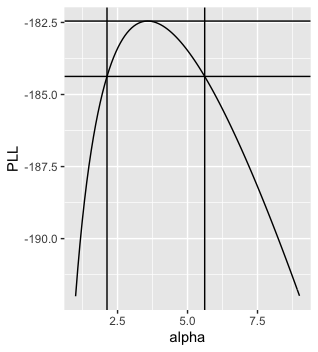
\includegraphics[width=1.5in]{a1/pll-alpha.png}}
\caption{Graph of the profile likelihood of $\alpha$ parameter in Gamma model}
\end{center}
\end{figure}
Let $\alpha_0$ be the true value of our alpha parameter. Using the profile deviance to create the confidence interval, we get \[\alpha_0\in [2.122419,5.612549]\]
Since 2 is not in this interval, we reject the null hypothesis.

\begin{figure}[H]
\begin{center}
{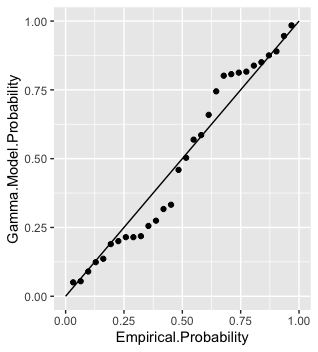
\includegraphics[width=2in]{a1/gamma-pp.png}}
{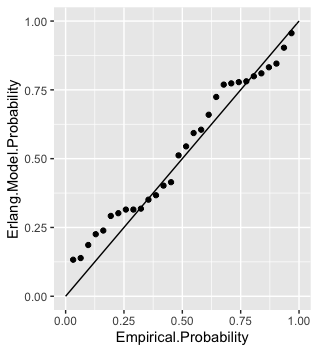
\includegraphics[width=2in]{a1/erlang-pp.png}}
\caption{P-P plots for Gamma model (left) and Erlang model (right)}
\end{center}
\end{figure}

\begin{figure}[H]
\begin{center}
{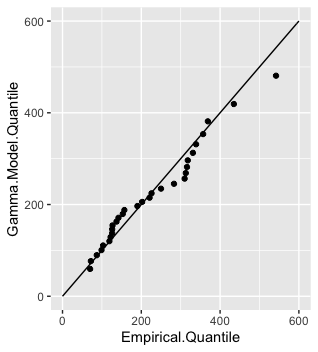
\includegraphics[width=2in]{a1/gamma-qq.png}}
{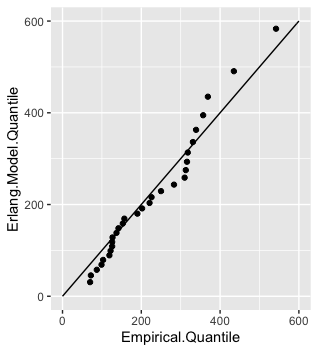
\includegraphics[width=2in]{a1/erlang-qq.png}}
\caption{Q-Q plots for Gamma model (left) and Erlang model (right)}
\end{center}
\end{figure}

In line with our hypothesis test, the model diagnostics seem to confirm that an Erlang(2) model is not enough to capture the complexity of our data. The overlap between our model  and empirical probabilities is higher in the P-P plot of the Gamma model. Similarly, the overlap of the quantiles is  higher in the Gamma model. We also observe from the Q-Q plots that the Gamma model better captures the tail behavior of our observed data.
\end{solution}

\begin{problem}{1}
\section*{Part A}
Fit the following model to the execution times (in seconds) of sell orders in \texttt{assn1P2.csv}:
\[f(y; \lambda) = \lambda \exp\bigg\{-\lambda(y - \frac{1}{2})\bigg\},\hspace{1cm} y \geq 1/2, \lambda > 0\tag{1}\]
Compute
\begin{enumerate}
    \item a 95\% confidence interval based on asymptotic normality;
    \item a 95\% confidence interval based on the deviance;
\end{enumerate}

for the 0.99 quantile of the execution time of sell orders based on the model in (1). Comment.

\section*{Part B}
When estimating the 0.99 quantile of the model in (1), can confidence intervals based on
asymptotic normality and confidence intervals based on profile likelihood be the same? Make
your point using simulated data.
\end{problem}
\begin{solution}
\section*{Part A}
Let us recover the analytical form of the quantile function corresponding to model (1). To do this, we first find the cdf:
\begin{align*}
    f(y;\lambda)&=\lambda \exp\bigg\{-\lambda(y-\frac{1}{2})\bigg\}\hspace{1cm} y \geq 1/2, \lambda > 0\\
    \implies F(y;\lambda)&= \int_\frac{1}{2}^y\lambda \exp\bigg\{-\lambda(y-\frac{1}{2})\bigg\}dy\\
    &=\lambda e^\frac{\lambda}{2}\bigg\{ \frac{-e^{-\lambda y}}{\lambda}\bigg|_{\frac{1}{2}}^y\bigg\}\\
    &=1-e^{-\lambda (y-\frac{1}{2})}
\end{align*}
Now, we find the quantile function $Q(p)$ by inverting the cdf
\begin{align*}
    p&=1-e^{-\lambda (y-\frac{1}{2})}\\
    \implies Q(p;\lambda)&=\frac{-\log(1-p)}{\lambda}+\frac{1}{2}
\end{align*}
Since this is a function of $\lambda$, we can estimate $Q(0.99)$ with \[\hat{Q}(0.99)=Q(0.99, \hat{\lambda})= \frac{-\log(0.01)}{\hat{\lambda}}+\frac{1}{2}\]
Next, we $\hat{\lambda}$ find using the maximum likelihood estimate:
\begin{align*}
    \mathcal{L}(\lambda)&=\prod_{i=1}^{20}\lambda \exp\bigg\{-\lambda(y_i-\frac{1}{2})\bigg\}\\
    \l(\lambda)&=\sum_{i=1}^{20} \log(\lambda)-\lambda y_i + \frac{\lambda}{2}\\
    \frac{\pt }{\pt \lambda}\l(\lambda)&= \frac{20}{\lambda}+10-\sum_{i=1}^{20}y_i\\
    \implies \hat{\lambda}&=\frac{20}{-10+\sum_{i=1}^{20}y_i}=0.1654944\\
    \implies \hat{Q}(0.99)&=28.32674
\end{align*}
Once we have our estimate, we can use the observed information matrix to recover it's variance:
\begin{align*}
    \fish_{O}(\lambda)&= -\frac{\pt^2}{\pt \lambda^2}\l(\lambda)\bigg|_{\lambda=\hat{\lambda}}\\
    &=-\frac{\pt }{\pt \lambda}\bigg[ \frac{20}{\lambda}+10-\sum_{i=1}^{20}y_i \bigg]\bigg|_{\lambda=\hat{\lambda}}\\
    &=\frac{20}{\hat{\lambda}^2}\\
    \implies Var(\hat{\lambda})&=\frac{\hat{\lambda}^2}{20}=0.00136941
\end{align*}
In the case of asymptotic normality, we can use the delta method to find the variance of $\hat{Q}(0.99,\hat{\lambda})$:
\begin{align*}
    \frac{\pt}{\pt \lambda}Q(p,\lambda)&= \frac{\log(1-p)}{\lambda^2}\\
    V_{\hat{Q}(0.99,\hat{\lambda})}&= \frac{\log(0.01)^2}{\hat{\lambda}^4}Var(\hat{\lambda})=\frac{\log(0.01)^2}{20\hat{\lambda}^2}=38.71
\end{align*}
Now we can calculate the asymptotically normal confidence interval for the quantile:
\[ 28.32674 \pm 1.96 \sqrt{\frac{ V_{\hat{Q}(0.99,\hat{\lambda})}}{20}} =[25.60,31.05]\]

In the case of a confidence interval derived from deviance, we take  different route. First, let us write $\lambda$ as a function of what we wish to build a CI for: $q=Q(0.99,\lambda)$:
\[\lambda(q)=\frac{-\log(0.01)}{q- \frac{1}{2}}\]

Next, we substitute $\lambda(q)$ into our likelihood function and observe how $q$ affects our likelihood:
\[\l(q)=\sum_{i=1}^{20} \log(\lambda(q))-\lambda(q) y_i + \frac{\lambda(q)}{2}\]
From this manipulation, we get 
\[Q(0.99) \in [18.99581,45.1453]\]
\begin{figure}[H]
\begin{center}
{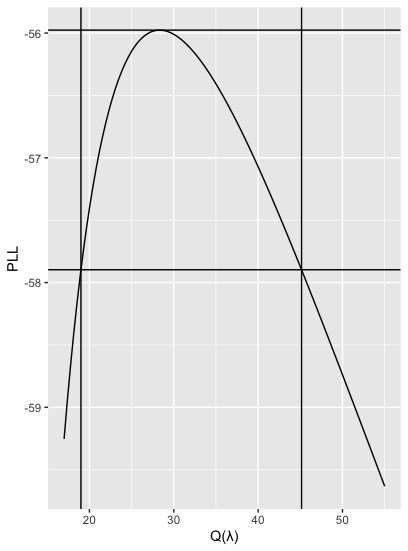
\includegraphics[width=2in]{a1/pll-lambda.png}}
\caption{Graph of the profile likelihood of $\lambda$ as a function of $Q(\lambda)$}
\end{center}
\end{figure}

\section*{Part B}
After finding confidence intervals for data simulated using the quantile function and random draws from the uniform distribution, we believe that the intervals based asymptotic normality and profile likelihood cannot be the same. In fact, we see that often our normal confidence intervals fail to capture the true value. 
\begin{figure}[H]
\begin{center}
{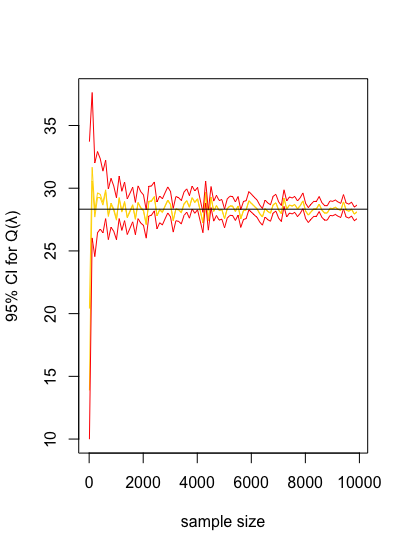
\includegraphics[width=2in]{a1/graph1.png}}
\caption{Confidence intervals derived from asymptotic normality (yellow) and profile deviance (red). The true value of $Q(\lambda)$ is show as the black line. Here, we can visualise the comparatively high failure rate of the confidence intervals de
rived from asymptotic normality. }
\end{center}
\end{figure}


\begin{figure}[H]
\begin{center}
{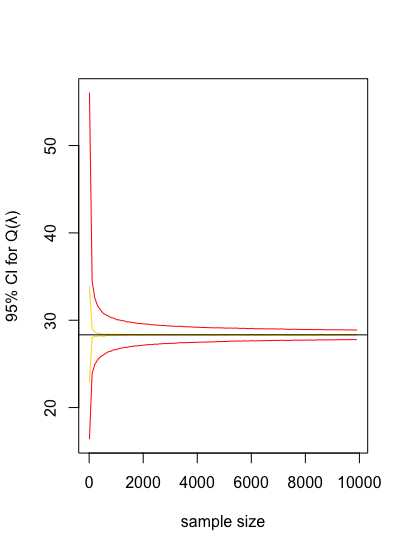
\includegraphics[width=2in]{a1/graph2.png}}
\caption{Average of 1000 confidence intervals derived from asymptotic normality (yellow) and profile deviance (red).}
\end{center}
\end{figure}
From both the graphs above, we theorize that although both confidence intervals bounds (at least when we average out experiments) converge to the true value, they will never be the same. 


\end{solution}



\end{document}

